\section{Sesión 19}

\subsubsection{Diferenciacion en $\mathbb{R}^n$}

Sea $F:X\subseteq \mathbb{R}\to\mathbb{R}\implies F$ es diferenciable en $x=a\in X$ significa que la gráfica de $F$ tiene un recta tangente en $(a,F(a))$,  



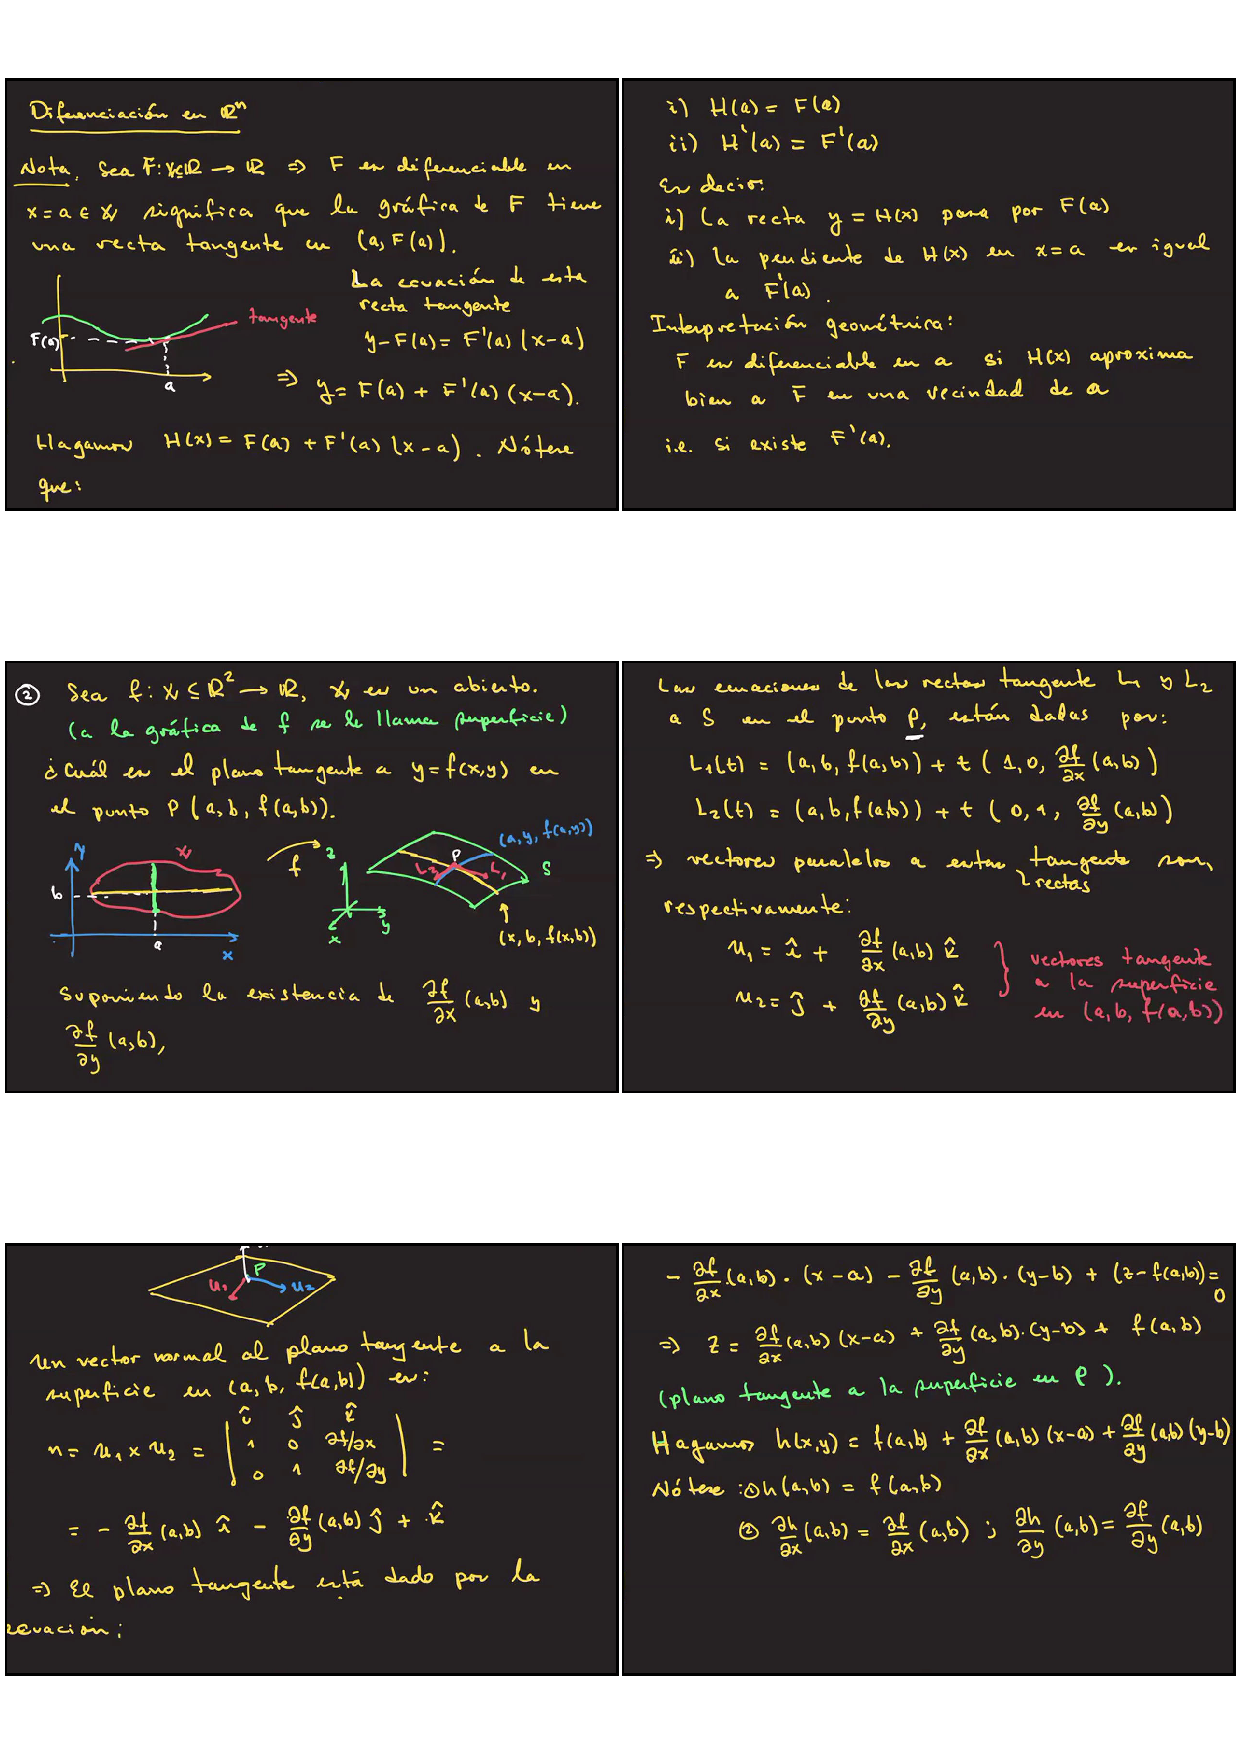
\includepdf[pages=-]{apendices/s19.pdf}